\documentclass[CJKutf8,dvipsnames,table]{beamer}
\usepackage{hyperref}
\hypersetup{
  pdfpagemode={FullScreen},
  colorlinks={true},
  linkcolor={blue},
}

%% https://tex.stackexchange.com/questions/47576/combining-ifxetex-and-ifluatex-with-the-logical-or-operation
\usepackage{iftex}
\newif\ifxetexorluatex % a new conditional starts as false
\ifnum 0\ifxetex 1\fi\ifluatex 1\fi>0
   \xetexorluatextrue
\fi
\usepackage{ifplatform}
\ifxetexorluatex
	\usepackage[slantfont,boldfont]{xeCJK}
	\ifwindows
		\setCJKmainfont{SimSun} % Windows默认中文字体:中易宋体
	\fi
	\ifmacosx
		\setCJKmainfont{STSong} % MacOS默认中文字体:华文宋体
	\fi
	\iflinux
		\setCJKmainfont{Noto Serif CJK SC} % Linux默认中文字体:思源宋体(By Adobe & Google)
	\fi
\else
	\usepackage{CJKutf8}
\fi

\usepackage[export]{adjustbox}
\usepackage{mathptmx} %pdfTeX error: pdflatex (file fmex9.pfb): cannot open Type 1 font file for reading
                                                 %https://forum.ubuntu.com.cn/viewtopic.php?t=269943

\usetheme{Madrid}%{Warsaw}
\usecolortheme{default}

\setbeamertemplate{footline}[page number]{} %gets rid of bottom navigation bars
\setbeamertemplate{navigation symbols}{} %gets rid of navigation symbols

\title{数字信号处理}
\subtitle{第3章:系统}
\author{洪明坚}
\institute{重庆大学软件学院}
\date{\today}

\begin{document}
\ifxetexorluatex\else
\begin{CJK*}{UTF8}{song}
\fi

  \AtBeginSection[]
  {
    \begin{frame}
      \frametitle{Outline}
      \tableofcontents[currentsection]
    \end{frame}
  }

  \frame{\titlepage}
  \frame{\frametitle{目录}\tableofcontents}
  
  \section{系统}
  
  %% PAGE
  \begin{frame}
    \frametitle{定义}
    \begin{itemize}
    \item 一个系统接受一定的输入,经过处理后,产生一些输出。
        \begin{itemize}
        \item $y=T(x)$,$x$是输入,$y$是输出
        \end{itemize}    
    \end{itemize}
    \begin{center}
      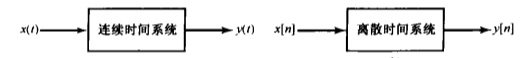
\includegraphics[scale=.5]{ss-c-f1-41}
    \end{center}    
  \end{frame}

  %% PAGE
  \begin{frame}
    \frametitle{例子}
    \begin{itemize}
    \item RC电路
    \begin{center}
      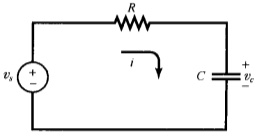
\includegraphics[scale=.5]{ss-c-f1-1}
    \end{center}       
        \begin{itemize}
        \item 输入$v_s(t)$与输出$v_c(t)$之间的关系:$\frac{dv_c(t)}{dt}+\frac{1}{RC}v_c(t)=\frac{1}{RC}v_s(t)$
        \end{itemize}  
    \item 银行存款
        \begin{itemize}
        \item 输入(存款)$x[n]$与输出(当前余额)$y[n]$之间的关系:$y[n]=(1+r)y[n-1]+x[n]$,r是利率
        \end{itemize}      
    \end{itemize} 
  \end{frame}

  %% PAGE
  \begin{frame}
    \frametitle{系统互联}
    \begin{itemize}
    \item 复杂的系统可以由简单的系统互联(interconnect)形成。几种常见的互联方式:
        \begin{itemize}
        \item 串联(series/cascade)
    \begin{center}
      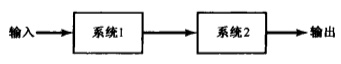
\includegraphics[scale=.5]{ss-c-f1-42a}
    \end{center}           
        \item 并联(parallel)
    \begin{center}
      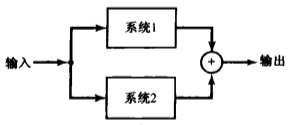
\includegraphics[scale=.5]{ss-c-f1-42b}
    \end{center}           
        \item 反馈(feedback)
    \begin{center}
      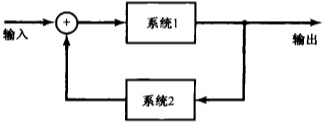
\includegraphics[scale=.5]{ss-c-f1-43}
    \end{center}           
        \end{itemize}    
    \end{itemize} 
  \end{frame}
      
  %% PAGE
  \begin{frame}
    \frametitle{系统属性}
    \begin{itemize}
    \item 记忆性:如果系统的输出仅仅取决于该时刻的输入,则无记忆
        \begin{itemize}
        \item 无记忆系统(memoryless)
            \begin{itemize}
            \item 恒等(identity)系统:$y(t)=x(t)$
            \item 缩放系统:$y(t)=Cx(t)$
            \end{itemize}
        \item 有记忆系统   
            \begin{itemize}
			\item 累加器(accumulator):$y[n]=\sum_{k=-\infty}^{n}x[k]=y[n-1]+x[n]$
            \item 延迟单元(delay):$y[n]=x[n-1]$
            \end{itemize}
        \end{itemize}       
    \item 可逆性:如果系统不同的输入产生不同的输出,则可逆
        \begin{itemize}
        \item 不可逆系统
            \begin{itemize}
            \item $y(t)=x^2(t)$
            \item $y[n]=0$
            \end{itemize}
        \item 可逆系统(invertible)    
            \begin{itemize}
            \item $y(t)=2x(t)$的逆是$w(t)=\frac{1}{2}y(t)$
	   \item 累加器$y[n]=y[n-1]+x[n]$的逆是$w[n]=y[n]-y[n-1]$
            \end{itemize}
        \end{itemize} 
    \end{itemize} 
  \end{frame}

  %% PAGE
  \begin{frame}
    \frametitle{系统属性(续)}
    \begin{itemize}
    \item 因果性:如果系统的输出只取决于现在及过去的输入,则因果
        \begin{itemize}
        \item 非因果
            \begin{itemize}
            \item $y(t)=x(t+1)$
            \item $y[n]=x[n]-x[n+1]$
            \end{itemize}
        \item 因果(causal)    
            \begin{itemize}
            \item 恒等系统
	   \item 累加器$y[n]=y[n-1]+x[n]$
            \end{itemize}
        \item $y(t)=x(t)cos(t+1)$是否因果?
        \end{itemize}     
    \item 稳定性:如果系统的输入是有界的,其输出也是有界的,则稳定
        \begin{itemize}
        \item 不稳定
            \begin{itemize}
            \item $y(t)=tx(t)$
            \item 累加器
            \end{itemize}
        \item 稳定(stable)    
            \begin{itemize}
            \item $y(t)=e^{x(t)}$
	   \item 恒等系统
            \end{itemize}
        \end{itemize}     
    \end{itemize} 
  \end{frame}

  %% PAGE
  \begin{frame}
    \frametitle{系统属性(续)}
    \begin{itemize}
    \item 时不变性:如果输入有一个时移,输出产生相同的时移,即$y(t-t_0)=T(x(t-t_0))$,则时不变
        \begin{itemize}
        \item 时变
            \begin{itemize}
            \item $y(t)=x(2t)$
            \item $y[n]=nx[n]$
            \end{itemize}
        \item 时不变(time invariant)    
            \begin{itemize}
            \item $y(t)=sin[x(t)]$
            \end{itemize}
        \end{itemize}        
    \item 线性:
          \begin{itemize}
          \item 如果系统满足以下两个条件,则线性
          \begin{itemize}
          \item 可加性(additivity):$y_1(t)+y_2(t)=T(x_1(t)+x_2(t))$
          \item 齐次性(homogeneity):$ay(t)=T(ax(t)), \forall a \in \mathbb{C}$
         \end{itemize}
          \end{itemize}
        \begin{itemize}
        \item 非线性(non-linear)
            \begin{itemize}
            \item $y(t)=x^2(t)$
            \item $y[n]=Re\{x[n]\}$
            \end{itemize}
        \item 线性(linear)    
            \begin{itemize}
            \item $y(t)=tx(t)$
            \item $y[n]=2x[n]$
            \end{itemize}
        \item $y[n]=2x[n]+3$是否线性?
        \end{itemize}  
    \end{itemize} 
  \end{frame}
        
  %% PAGE
  \begin{frame}
    \frametitle{Questions}
    \begin{itemize}
    \item Any questions?
    \end{itemize}
    \begin{center}
      
\includegraphics[scale=.5]{question}
    \end{center}
  \end{frame}    
  
  \section{线性时不变系统}
  
  %% PAGE
  \begin{frame}
    \frametitle{线性时不变系统(LTI)}
    \begin{itemize}
    \item 特别重要
        \begin{itemize}
        \item 很多物理过程满足线性和时不变性
        \item 可以对LTI系统进行详细的分析
        \end{itemize}   
    \end{itemize} 
  \end{frame} 
  
  %% PAGE
  \begin{frame}
    \frametitle{LTI系统的单位冲激响应}
    \begin{itemize}
    \item 单位冲激信号
    
    \begin{math}
\delta[n] = 
\left\{
    \begin {aligned}
         & 0 \quad & n \neq 0 \\
         & 1 \quad & n = 0                  
    \end{aligned}
\right.
	\end{math}    
 
    \item 采样功能
        \begin{itemize}
        \item 
    \begin{math}
x[k]\delta[n-k] = 
\left\{
    \begin {aligned}
         & 0 \quad & k \neq n \\
         & x[n] \quad & k = n                  
    \end{aligned}
\right.
	\end{math}     
        \item $x[n]=\sum_{k=-\infty}^{\infty}x[k]\delta[n-k], \forall n \in \mathbb{Z}$
        \end{itemize} 
        
    \item $y[n]=T(x[n])=T(\sum_{k=-\infty}^{\infty}x[k]\delta[n-k])$
        \begin{itemize}
        \item 根据线性,有$y[n]=\sum_{k=-\infty}^{\infty}x[k]T(\delta[n-k])$
        \item 根据时不变性,有$y[n]=\sum_{k=-\infty}^{\infty}x[k]h[n-k]$
            \begin{itemize}
            \item 其中,$h=T(\delta)$
            \end{itemize}
        \end{itemize}
    \item 对于LTI系统,任意输入的响应可以用单位冲激响应$h$来表示,即单位冲激响应完全刻画了LTI系统的特征。
    \end{itemize} 
  \end{frame}    
    

  \section{卷积}
      
  %% PAGE
  \begin{frame}
    \frametitle{卷积(Convolution)}
    \begin{itemize}
    \item 定义
        \begin{itemize}
        \item 序列$x_1$与$x_2$的卷积:$(x_1*x_2)[n]=\sum_{k=-\infty}^{\infty}x_1[k]x_2[n-k], \forall n \in \mathbb{Z}$
        \end{itemize}   
    \item 因此,LTI系统输出是输入$x$与单位冲激响应$h$的卷积
    \end{itemize} 
  \end{frame}     
    
\ifxetexorluatex\else
\end{CJK*}
\fi
\end{document}

%%% Local Variables: 
%%% mode: latex
%%% TeX-master: t
%%% End: 
